\documentclass[a4paper,12pt]{article}
\usepackage[backend=biber, citestyle=authoryear, bibencoding=utf8]{biblatex}
\addbibresource{../bibs/external-validity.bib}
\addbibresource{../bibs/econ-causal-history.bib}
\addbibresource{../bibs/causality.bib}
\addbibresource{../bibs/domain-adaptation.bib}
\addbibresource{../bibs/economic-forests.bib}
\addbibresource{../bibs/microcredit.bib}
\addbibresource{../bibs/extra-citations.bib}
\addbibresource{../bibs/quantile-regression.bib}
\addbibresource{../bibs/cash-transfers.bib}

\usepackage{amsmath, amsthm, amsfonts, mathtools, csquotes, bm, centernot, bbm}

\usepackage[default,light,bold]{sourceserifpro}
\usepackage[T1]{fontenc}

\newtheorem{prop}{Proposition}

\usepackage{pgf, tikz}
\usetikzlibrary{arrows, automata}

\DeclareMathOperator*{\argmax}{argmax}
\DeclareMathOperator*{\argmin}{argmin}
\DeclareMathOperator*{\D}{\mathcal{D}}



\newcommand{\CI}{\mathrel{\perp\mspace{-10mu}\perp}}
\newcommand{\nCI}{\centernot{\CI}}

\title{ Policy Prediction Across Contexts  }

\author{Nandan Rao}


\begin{document}

\maketitle

\begin{abstract}
Applied economics research is most often ``applied'' to policy making. In the literature on experimental and quasi-experimental econometrics, however, there are few formal frameworks that use the results of experimental studies to predict the effects of policies in new contexts. This research agenda lays out a plan to fill this gap using recent ideas from econometrics and machine learning. I will also explain the existence of the gap from a historical perspective and review the current methods that do exist to motivate the research I am proposing.
\end{abstract}

\clearpage

\tableofcontents

\clearpage

\section{Introduction}

Randomized control trials (RCTs), or natural experiments that replicate them, have become the official gold standard of empirical work in economics and many related fields. More and more, policy makers are encouraged to look to RCTs to make ``evidence-based'' policy decisions (\cite{Manski2013, Cartwright2013}).

Many prominent economists have expressed a concern that RCTs and their quasi-experimental colleagues (i.e. natural experiments, instrumental variables, regression discontinuity, etc.) are particularly difficult to generalize to new contexts due to their overarching concern for internal validity, often at the expense of external validity (\cite{Heckman1995, Heckman2008, Deaton2010, Manski2013, Deaton2018}).

Making evidence-based policy decisions is an act of generalizing from previous studies to decisions about the future. Charles Manski \parencite*{Manski2013} voices the concern that experimental studies have tended to ``be silent'' on the question of external validity and that ``from the perspective of policy choice \ldots What matters is the informativeness of a study for policy making, which depends jointly on internal and external validity.''

This silence on external validity means that, despite the huge field of research and techniques for ensuring causal identification (internal validity) via experimental or quasi-experimental methods, very little has been done to either A) create tools to prove that the same results will apply generally in all contexts or B) create tools to predict the results in a specific context, given proven results from one or more experiments.

Abhijit Banjerjee himself \parencite*{Snowberg2016}, a large proponent of RCTs, has recently echoed the current lack of and need for more formal systems for the generalization of experimental studies, stating ``it is our belief that creating a rigorous framework for external validity is an important step in completing an ecosystem for social science field experiments, and a complement to many other aspects of experimentation.''

In response to such theoretical concerns, a small but growing literature  has sprung up around empirically proving that results from prominent RCT or other causally identified studies do not easily extrapolate to new contexts (\cite{Pritchett2016, Allcott2015, Bisbee2017, Rosenzweig2019}). These results emphasize a need for powerful extrapolation tools if policy makers are realistically expected to make decisions based on ``evidence.''

Predicting the results of a policy in a new location is, tautologically, a prediction problem. Machine learning is a field which has been very successful at formalizing prediction problems. Domain adaptation, a subfield of machine learning, formalizes the problem of moving from one (or more) domains with labelled data to a new domain where only unlaballed data is available (\cite[for a survey, see][]{Pan2010}).

Formulating the problem of policy prediction in terms of domain adaptation provides a rigorous way to think about the assumptions that may or may not hold, as well as a rich (if short) history of techniques that have been used to solve the problems associated with those assumptions. I will show how policy prediction can be formulated as a covariate shift problem and propose that the associated assumptions could be tested empirically in a treatment effects framework.

This research proposal will take the following form. First I will lay out the high-level aims, research question, and deliverables. Following that, I will provide the basic theoretical background necessary to prove that my research agenda is feasible. I will then provide an outline of the three articles that will make up each chapter of my thesis. Finally, I will provide a timeline that covers the next 2 years of the project.


\section{Research Objectives and Questions}

The focal question of this research is: \textit{given a set of causally-identified treatment-effect studies in different contexts, how can one predict the treatment effect in a new context}?

A full motiviation and overview of related literature will be provided in the following section, however I provide some simple intuition here to highlight the novelty of this question.

Consider that, given a set of data from a single study, one learns a conditional distribution of the treatment effect $P(\tau | X)$. Often one might report the expected value of this distribution, where the expectation is taken over the marginal distribution of covariates in the study location, $P(X)$. This returns the average treatment effect (ATE) $\int P(\tau | X)P(X) dX$. If the conditional treatment effect, $P(\tau | X)$ were constant between the context of the study and the desired prediction context, then one can reintegrate over the marginal distribution of covariates in the target context to gain a predicted ATE.

Trivially, we can always write the conditional treatment effect as an integral over the unobserved variables that are not included in the covariates:
%
$$
P(\tau | X) = \int P(\tau | X, H) P(H | X) dH
$$
%
Having expanded our conditional treatment effect thus, it becomes obvious that the assumption needed for transportability of this distribution is stability of $P(H | X)$ (see \cite{Pearl2014} for a full characterization of transportability in a more general setting). One can then use this stability assumption as a search criter to find a model ($P(\tau | X)$) that will provide the best predictions in a new context.

This is a relatively new line of research in the statistics and machine learning communities (\cite{Rojas-carulla2018, Heinze-deml2017}), but there are two aspects missing which are of critical importance to economic research: A) an explicit handling of treatment effects, treatment effect heterogeneity, and the high-dimensional variable selection problem that is created and B) an explicit investigation into the case of latent variables and their proxies, as often occurs in the social sciences.

I propose a series of 3 articles which lay out new econometric techniques aim at extending these ideas into this new context and test the new techniques empirically:

\begin{enumerate}
\item Predicting Treatment Effects in a New Context: A Sparse Linear Model.
\item Predicting Treatment Effects in a New Context: A Non-Linear Decision Tree Model.
\item Predicting the Effects of Unconditional Cash Transfer Programs Across Countries
\end{enumerate}

\section{ Background Literature and Motivation }

\subsection{Validity and Counterfactual Identification}

\subsubsection{A Taxonomy of Validities}

Critiques against the holy status of RCTs have focused on the proponents' preference for internal validity and tendency to completely ignore external validity (\cite{Manski2013, Deaton2018}). It is worth defining these terms and reflecting on exactly what it is that experimental methods provide us. The most agreed upon definition of these terms comes from \cite{Shadish2002} (an update of their previously popular taxonomy of validities from \cite{Cook1979}):

\begin{displayquote}
\textbf{Statistical Conclusion Validity:} The validity of inferences about the correlation (covariation) between treatment and outcome.

\textbf{Internal Validity:} The validity of inferences about whether observed covariation between A (the presumed treatment) and B (the presumed outcome) reflects a causal relationship from A to B as those variables were manipulated or measured.

\textbf{Construct Validity:} The validity of inferences about the higher order constructs that represent sampling particulars.

\textbf{External Validity:} The validity of inferences about whether the cause-effect relationship holds over variation in persons, settings, treatment variables, and measurement variables.
\end{displayquote}

Many authors use the term external validity to refer to what Shadish, Cook, and Campbell separate into construct and external validity. As both are involved in generalization, and both are external to the particulars of the sample, I will follow that abuse of terminology and refer to all the challenges of both as ``external validity.''

What, then, is meant by the term ``inference?''

\subsubsection{Inference and Statistics}

Mary S. Morgan, in her \textit{History of Econometric Ideas} \parencite*{Morgan1991}, lays out the tension between mathematics and statistics in economics of the nineteenth-century: mathematics was seen as a tool for deductive reasoning, used to derive logical conclusions from known laws while statistics, on the other hand, was viewed as a tool for inductive reasoning, used to establish economic regularities.

This distinction between deduction and induction follows from the Aristotelian tradition of logic, where inference is the process of reasoning and can be broken into two parts: reasoning from particulars to generals (induction) and reasoning from generals to particulars (deduction). Once one has induced a general law (``all men are mortal''), one can deduce facts that might otherwise not yet be apparent (``Socrates will die''). There is, of course, a natural contradiction in this process: how can one know that all men are mortal, if one did not already know that Socrates will die? In other words, how can one ever claim that ``all men are mortal'' until one has seen every man die?

This problem forms the foundation of David Hume's \textit{Problem of Induction}:

\begin{displayquote}
``As to past Experience, it can be allowed to give direct and certain information of those precise objects only, and that precise period of time, which fell under its cognizance: but why this experience should be extended to future times, and to other objects, which for aught we know, may be only in appearance similar, this is the main question on which I would insist'' \parencite{hume1748}
\end{displayquote}

There are two distinct problems Hume raises, that of generalizing from one object to another (from seeing some men die to assuming all men have died) and that of generalizing from the past to the future (because all men have died, thus, all men will die). He goes on to explain that this extrapolation is only valid under strong assumptions as to the ``uniformity of nature.'' One must assume nature is uniform in such a way as to enable extrapolation from one object to another or from the past to the future.

R.A. Fisher also framed his statistical techniques in terms of ``inductive inference.'' In the introduction to \textit{The Design of Experiments} \parencite*{Fisher1935}, he explicitly frames his canonical book and its techniques in the terms of logicians such as Hume, arguing for the possibility of induction via statistical methods:
%
\begin{displayquote}
``\ldots it is possible to draw valid inferences from the results of experimentation\ldots as a statistician would say, from a sample to the population from which the sample was drawn, or, as a logician might put it, from the particular to the general.'' \parencite{Fisher1935}
\end{displayquote}

Fisherian statistical inference is a tool in the process of induction that seeks to address Hume's problem of extending experience with one object to that of similar objects. In particular, the ``similar objects'' to which conclusions are extended are not just similar in appearance, but rather have a distinct relationship to the experienced objects: they are the population from which the experienced objects represent a sample.

Fisher's methodologies for significance testing relate to drawing conclusions about populations given a sample. The validity of the use of such techniques in a study falls squarely under the category of ``statistically conclusion validity'' in the taxonomy of Shadish, Cook, and Campbell.

Fisher's theory of experiments (in particular, the RCT) addresses internal validity and causality. The connection between the RCT and the identification of a causal relationship comes straight from John Stuart Mill's \parencite*{mill1884} \textit{Method of Difference} for causal discovery:

\begin{displayquote}
  ``If an instance in which the phenomenon under investigation occurs, and an instance in which it does not occur, have every circumstance save one in common, that one occurring only in the former; the circumstance in which alone the two instances differ, is the effect, or cause, or a necessary part of the cause, of the phenomenon.''
\end{displayquote}

Fisher \parencite*{Fisher1935} had this in mind when he defended randomization, claiming that holding all other variables constant was not feasible, and thus, holding them to the same distribution, by making the assignment of treatment independent of those variables, was desirable (\cite{Rosenbaum2005}). It should be noted, however, that for the subjects of interest to Fisher, the difference between something being a ``cause'' or ``a necessary part of the cause'' was not especially important. What Fisher was interested in was essentially interventional prediction: what are the effects of a given cause (individual changes to the growing conditions of these plants).

Holland \parencite*{Holland1986} begins his landmark paper, before formulating the Rubin-Neyman causal model, by framing his goal:

\begin{displayquote}
``Others are concerned with deducing the causes of a given effect. Still others are interested in understanding the details of causal mechanisms. The emphasis here will be on measuring the effects of causes because this seems to be a place where statistics, which is concerned with measurement, has contributions to make.''
\end{displayquote}

The success of Fisher's framework of randomization and the Rubin-Neyman causal model comes down to this razor focus in purpose: they make no claims to discover all the causes of a given effect, to discover the mechanism of the cause, or even to separate between a cause or a necessary part of a cause. They allow us to reason about counterfactuals: what would have happened, on average and in the past, had we treated our entire population rather than a randomized part of a randomized sample drawn from that population. It operationalizes Mill's method of differences, creating a pathway to internal validity that is achievable in the real world.

The counterfactual causal model, however, provides no framework for generalizing from a specific population to a more general one or from the past to the future (\cite{Heckman2008}). The ``effects of causes'' is a black-box methodology for causal identification  (\cite{Heckman1995}). It does not require one to answer the question ``why'' and it is therefore inherently context specific: it asks, ``what happened when I did $X$ in context $D$?'' In Fisher's line of work (agriculture), none of those shortcomings were problematic. He was able to randomly sample from the exact population (seeds of grain) to which his inferences needed to generalize.

The success of Fisher's randomization in his field of agriculture, and the subsequent success of the Rubin-Neyman causal model in epidemiology, is in no way incidental. These are fields that deal with encapsulated biological units where agreed-upon scientific theory tells us that the relationships in these systems will be invariant to a wide degree of changes that happen in the world from one year to the next or from one country to the next.

For example, it is implicitly assumed that the growth of corn will not be affected by its expectations of how it will be cut down and processed during the harvest. Corn grows according to the properties of the soil and the sun it receives. Its growth will be independent of its destination in corn flakes or arepas, conditional on those properties. Opioids will inhibit pain in humans, regardless of their political ideology, faith in their governmental institutions, or their love of Shark Tank.

These arguments are not made explicitly, but their validity is absolutely necessary to enable the application of their findings: they create laws defined in relation to the entire range of contextual changes that one might want for prediction- and decision-making and that allows the laws to be applied deductively in a wide array of useful situations.

While the validity of these arguments is taken for granted in contained biological processes, this is simply not the case in the social sciences. This is why Shadish, Cook, and Campbell lay out 19 different threats to construct and external validity of social science experiments. In the case of growing corn, the threats either simply do not apply or are implicitly neutralized through basic scientific understanding of plant growth.

In the case of economics, the outcomes are regularly based on individuals decisions to consume, work, study, invest, or move. The treatments are regularly subjected to a gauntlet of mediating factors and interacting variables that are highly context-dependent and correlated across individuals in a single place and time. The population for which one wants to draw actionable inference is in the future and that alone might make them fundamentally different in a number of relevant ways. Internal validity of a study in economics is not automatically sufficient for actionable inference to take place in a new context.

\subsubsection{The Danger of Informal Inference}

It might be argued that it is, and should be, up to the sound judgement and expert opinion of the policy maker to determine if a given counterfactual analysis should extrapolate to their context or not. Empirical studies only need to provide internal validity, according to this argument, as the extrapolation is done by experts who know their target domain.

While incorporating expert domain knowledge can only help predictions, we can differentiation between using a formal statistical framework and using an informal framework of judgement. John Stuart Mill \parencite*{mill1884}, reflects on these difference and the dangers of inferring without formal frameworks.

He begins by denying that the only process of inference consists of separately applying induction (particulars to generals) and then deduction (general law to particular context):

\begin{displayquote}
  ``All inference is from particulars to particulars: General propositions are merely registers of such inferences already made, and short formulae for making more: The major premise of a syllogism, consequently, is a formula of this description: and the conclusion is not an inferennnnce drawn from the formula, but an inference drawn according to the formula: the real logical antecedent, or premise, being the particular facts from which the general proposition was collected by induction.''  \parencite{mill1884}
\end{displayquote}

In other words, in the process of creating the general law, one has created a series of particular laws, and only once assured that all the particular laws are valid can one be assured of the more general law. He goes on to caution against the direct reasoning of particulars to particulars because it is informal and we are likely to bring our own biases into the process and make mistakes:
%
\begin{displayquote}
``In reasoning from a course of individual observations to some new and unobserved case, which we are but imperfectly acquainted with (or we should not be inquiring into it), and in which, since we are inquiring into it, we probably feel a peculiar interest; there is very little to prevent us from giving way to negligence, or to any bias which may affect our wishes or our imagination, and, under that influence, accepting insufficient evidence as sufficient.'' \parencite{mill1884}
\end{displayquote}

John Stuart Mill argues that formal procedures, such as that implied by the framework of induction and deduction, allow individuals to avoid these biases. In his world, there was no formal procedure for reasoning from particulars to particulars, but there was for reasoning from particulars to general. As such, he recommends the latter as a way to avoid biases of ``wishes'' and ``imagination.''

In an ideal world, the research community has discovered a set of general laws that are invariant to all contexts and the policy maker can apply them, via the process of deduction, to get the desired result in their circumstance. But what if that general law has not yet been discovered? Then the policy maker must look at individual studies (particulars) and attempt to infer a prediction for the result of a similar policy in their context. This is exactly the situation that John Stuart Mill has warned is fertile ground for bias and imagination.

\subsection{The Origins of Structure}

Economists during the same period as Fisher took a different approach to conceptualizing and thinking about the inference they were doing. Ragnar Frisch, theorizing about macro-dynamic analysis, set out several key ideas relating to the structure of a system and the autonomy of a structure (\cite{Frisch1995}). For Frisch, the ``structure'' of a system was all the characteristics of the phenomena that could be quantitatively described. In his macrodynamic systems, the structure is defined by a set of functional (simultaneous) equations. He then poses the question: what would happen to the system due to an arbitrary change in a single variable? To do so could imply a different ``structure'' than the one which the equations describe, requiring a different set of equations altogether to describe the new system.

\begin{displayquote}
``But when we start speaking of the possibility of a structure different from what it actually is, we have introduced a fundamentally new idea. The big question will now be in what directions should we conceive of a possibility of changing the structure?\ldots To get a real answer we must introduce some fundamentally new information. We do this by investigating what features of our structure are in fact the most autonomous in the sense that they could be maintained unaltered while other features of the structure were changed\ldots So we are led to constructing a sort of super-structure, which helps us to pick out those particular equations in the main structure to which we can attribute a high degree of autonomy in the above sense. The higher this degree of autonomy, the more fundamental is the equation, the deeper is the insight which it gives us into the way in which the system functions, in short, the nearer it comes to being a real explanation. Such relations form the essence of 'theory'.''
\end{displayquote}

This concept, that of ``the essence of theory'' being the discovery of some relationship that is autonomous and invariant to a great degree of changes we can imagine performing to a system, is taken up by Trygve Haavelmo \parencite*{Haavelmo1944}, who writes that:

\begin{displayquote}
``The principal task of economic theory is to establish such relations as might be expected to possess as high a degree of autonomy as possible.''
\end{displayquote}

He then goes on to consider a distinction between the ``invariance'' of a relationship under hypothetical changes in structure versus the ``persistence'' of a relationship under observed changes in structure:

\begin{displayquote}
``\ldots if we always try to form such relations as are autonomous with respect to those changes that are in fact \textit{most likely to occur}, and if we succeed in doing so, then, of course, there will be a very close connection between actual persistence and theoretical degree of autonomy.''
\end{displayquote}

This implies a connection between autonomy and the \textit{type} of changes to which it is invariant \textit{with respect to}. This point is made even more explicitly by Leonid Hurwicz \parencite*{Hurwicz1966}. Similar to his predecessors, his model consists of a system of equations that constrain the state of the world, given a history of states. He calls this system of equations a ``behavior pattern.'' He states that:

\begin{displayquote}
``A great deal of effort is devoted in econometrics and elsewhere to attempts at finding the behavior pattern of an observed configuration\ldots But do we really need the knowledge of the behavior pattern of the configuration?\ldots It will be approached here from the viewpoint of prediction\ldots That is, the word `need' in the above question will be understood as `need' for purposes of prediction.''
\end{displayquote}

% He then goes on to explain that the need is driven by the type of prediction one hopes to make. If it can be assumed that the behavior pattern does not change (i.e. the joint distribution of our variables of interest comes from the same distribution tomorrow as today), then we do not actually need to find the behavioral pattern, as we can predict the state of the world tomorrow based on an expectation of the past.

He then goes on to define what he calls a ``structural form'' as one which is identified and identical across all possible behavior changes that one \textit{needs} to predict within. He stresses that:

\begin{displayquote}
``The most important point is that the concept of structure is relative to the domain of modifications anticipated.''
\end{displayquote}

Thus, there is an inherent and irrevocable connection between what we consider a ``law'' and the degree of changes we require the law to persist across. The law is defined in relation to those changes. Following Hume, the performance of induction is always connected to a specific assumption about the uniformity of nature. Additionally, the exact way in which nature must be uniform, for a particular system under study, is defined by the predictions we need to make with the discovered relations in that system.


\subsubsection{Invariant Conditionals}

Robert Engle, building on the work of Frisch and Hurwicz regarding invariant/autonomous structures, creates a statistical definition of what he terms ``super exogoneity'' (\cite{Engle1983}).A good review of this historical evolution of autonomy can be found in \cite{Aldrich1989}.

Super exogoneity is defined by Engle as follows. Consider a model in which the ``structure'' (the functional form) of a relationship between outcome $y$ and variable $z$ is parameterized by ``structural'' parameters $\lambda_1, \lambda_2 \in \lambda$. If the joint density implied by the model can be factorized as follows:
%
$$
P(y, z, \lambda) = P(y | z, \lambda_1)P(z | \lambda_2)
$$

and $\lambda_2$ is independent of, hence contains no information about, the structural parameter of interest $\lambda_1$, then the variable $z$ is said to be weakly exogenous to $\lambda_1$. If, additionally, the conditional distribution, $P(y | z, \lambda_1)$ remains invariant to changes in the marginal $p(z)$ (either caused by changes in it's generating process, parameterized by $\lambda_2$, or through other interventions that modify the values themselves), then $z$ is super exogenous.

This definition allows super exogoneity to be refuted by data:

\begin{displayquote}
``It is clear that any assertion concerning super exogeneity is refutable in the data for past changes in $D(z, | X_{t-1}, \lambda_2)$ by examining the behavior of the conditional model for invariance when the parameters of the exogenous process changed...However, super exogeneity for all changes in the distribution of z, must remain a conjecture until refuted, both because nothing precludes agents from simply changing their behavior at a certain instant and because only a limited range of interventions will have occurred in any given sample period.''
\end{displayquote}

This clarifies the difference between weak and super exogoneity: one is observational and the other interventional. Weak exogoneity is an observational characteristic, one must only show that structural parameters $\lambda_2$ provide no information for estimating $\lambda_1$. Super exogoneity implies invariance across any possible intervention which changes the distribution of $z$.

Writing a system in terms of super exogenous variables is akin to finding Frisch's ``super-structure.'' This is the part of the system that stays invariant to a set of allowable modifications: changes in $P(z)$. This is the part of the system that must be known in order to make policy predictions, where $z$ is changes directly or indirectly, whose total causal effect (\cite[in the sense of][]{Pearl2000}) is transmitted to the output variable $y$ through $z$. The existence of such an invariant super-structure is a necessary prerequisite to successfully predict the effects of policy and therefore to successfully inform policy choice from empirical data.

This method of looking in the data for a conditional distribution that is invariant to ``structural'' changes that lead to differences in the marginal distribution of its ``inputs'' has formed the basis of new line of work in statistics and machine learning around causal discovery (\cite{Peters2015, Heinze-deml2017, Rojas-carulla2018}). This line of research, in the terms of Engle, can be thought of as methods for model selection by selecting covariates that are super exogenous to the output in question. I will return to some of these methods in section 4.

Additionally, the connection between weak and super exogoneity is exploited by \cite{Zhang2015}, where the lack of weak exogoneity is used to determine the causal direction in the case of two correlated, unconfounded variables. Zhang's method points to the possibility of tests that exclude the assumptions of covariate shift with data from only a single domain. In other words, a general testing framework that works without testing directly for super exogoneity, which in theory requires proving the invariance of the conditional distribution $P(Y|Z)$ against all arbitrary manipulations of the marginal $P(Z)$.

% They work without making any assumption as to strong or weak exogeneity (\cite[in the sense of][]{Engle1983}) of the covariates, assumptions that are often provided by basic theory in economic contexts. Implications for further research based on such additional assumptions will be returned to in the sequel.

% It should be clear that, even if such a super-structure exists, it is possible that $z$ is either fully or partially unobserved. How will that effect the invariance? Consider again the model with a slight modification (we drop $\lambda_1$ for ease of notation, as we are only interested in the conditions under which the conditional distribution is invariant and thus $\lambda_1$ is static):
% %
% $$
% P(y, z_1, z_2, \lambda) = P(y | z_1, z_2)P(z_1 | z_2, \lambda_2)p(z_2 | \lambda_3)
% $$

% Where we consider a latent variable, $z_2$, which is independent of the policy modification of interest, $\lambda_2$, and whose generating process is controlled by structural parameter $\lambda_3$. We can marginalize out $z_2$ by fixing $\lambda_3 = \ell$:
% %
% $$
% P(y, z_1, z_2, \lambda_2, \lambda_3 = \ell_3) = P(y | z_1, \lambda_3 = \ell_3)P(z_1 | \lambda_2, \lambda_3 = \ell_3)
% $$

% Thus, our conditional is still invariant to modifications to $\lambda_2$, but it is fixed as regards the structural parameter $\lambda_3$ which determined the distribution of the latent variable $z_2$. If the latent variable, $z_2$, was also effected by the structural parameters $\lambda_2$, then one would have to fix that as well in order to get an invariant conditional:
% %
% $$
% P(y | z_1, \lambda_2 = \ell_2, \lambda_3 = \ell_3)
% $$

% It is worth considering the implications of the existence of latent variables in the super-structure that are evident in this simple exercise of probability algebra:

% \begin{enumerate}
% \item If the latent variable is not independent of the set of modifications to which a relationship should be invariant ($P(z | \lambda_2) \neq P(z)$), then the relationship cannot be determined generally.
% \item If the latent variable is independent of the set of modifications to which a relationship should be invariant ($P(z | \lambda_2) = P(z)$, then marginalizing out the latent variable results in an invariant relationship.
% \end{enumerate}

% This requirement is proved rigorously in \cite{Pearl2014}, where they refer to a relationship as ``transportable'' if it is invariant across a set of modifications.

% Given that $z_2$ is latent, it might be difficult, in practice, to know whether or not it is independent of $\lambda_2$: one cannot directly obtain an empirical estimate of $P(z_2)$. What about going in the reverse direction: if one had empirical data across a set of modifications (different values of $\lambda_2$) and one discovered an empirical conditional distribution $P(y | z_1)$ that is invariant across those modifications, does that imply that $P(z_2 | \lambda_2) = P(z_2)$?



\subsection{Domain Adaptation}

\subsubsection{Definition and Formulation}

Consider a domain, $\D$, which we define as consisting of a feature space, $\mathcal{X}$, and a marginal distribution $P(X)$ where $X = \{x_1,\ldots,x_n\} \in \mathcal{X}$. A task, $\mathcal{T}$, consists of an outcome space, $\mathcal{Y}$ and a true generating mechanism $f: \mathcal{X} \rightarrow \mathcal{Y}$.

Many techniques of traditional statistics and machine learning make the assumption that the domain and the task are the same in the training data and the prediction context. Transfer learning is the generic name for frameworks that work outside these assumptions, when either the domain, the task, or both are allowed to change.

I will consider the term domain adaptation in the sense of Ben-David \parencite*{Ben-David2006} and Pan and Yang \parencite*{Pan2010}. Under this definition, domain adaptation is a specific form of transfer learning where the task $\mathcal{T}$ is constant and the feature space, $\mathcal{X}$ is the same across all domains. There is a target domain, $\D_T$ from which one has samples $\{x_1,\ldots,x_n\} \in X$ and (one or more) source domain(s), $\D_S$, from which one has tuples $\{(y_1, x_1),\dots,(y_n, x_n)\} \in (\mathcal{Y}, \mathcal{X})$.

The consistency of the task relates to the construct validity in the taxonomy of \cite{Shadish2002}. If the outcome measured in one experiment might be considered to measure a different construct than the outcome measured in another experiment, then the task can not be said to be the same and this problem formulation fails.

Allow $\mathcal{X} = \{\mathcal{W}, \mathcal{Z}\}$, where $\mathcal{W} = \{W_0, W_1\}$ a binary treatment and $\mathcal{Z} = {Z_1,\ldots,Z_P}$ a set of covariates. The assumption of the consistency of the feature space relies on the construct validity of both the treatment and the covariates. If this validity does not hold, if the covariates or the treatment across domains represent a different construct, then this formulation is not valid.

If one considers a random-variable formulation of the true generating mechanism, $f(\cdot)$, then the assumption of task consistency implies the conditional distribution is consistent across tasks, thus $P_S(Y | X) = P_T(Y | X)$. This assumption is referred to as ``covariate shift'', as the only difference between domains $\D_S$ and $\D_T$ is that of the marginal covariate distribution, $P_S(X) \neq P_T(X)$.

Under the assumptions of covariate shift, Shimodaira \parencite*{Shimodaira2000} shows that the optimum likelihood function for a maximum likelihood estimator of $P_T(Y | X)$, given sufficiently large sample size, is obtained by minimizing the weighted loss function trained on labeled data from the source domain and weighted by the ratio $w(x) = \frac{P_T(x)}{P_S(x)}$:
%
$$
\argmin_{\beta} \sum_{i=0}^N -w(x_i) \log P_S(y_i | x_i, \beta)
$$

The use of this weighting ratio, $w(x)$ (referred to as the \textit{importance}) has led to many other importance estimation techniques to deal with covariate shift (\cite{Suigyama2007, Pan2010}).

For the rest of this article, I will focus on the goal of formulating policy prediction problems such that the covariate shift assumption holds. If that assumption holds, the task of policy prediction in a new context can be solved with a relatively straight-forward application of importance estimation techniques.

\subsubsection{Domain Adaptation in Econometrics}

The problem of covariate shift has a related, long history in the problem of overcoming sample selection bias in econometrics (\cite{Manski1977}). While the fundamental statistical problem is the same, the applications are specific.

The most obvious economic approach which addresses the problem of external validity is that of structural economics. Heckman \parencite*{Heckman2008} explains that RCTs solve internal validity, while the problem that ``economic policy analysts have to solve daily'' involves more, and not just the generalization of previous experiments but also the prediction of the effects of policies ``never historically experienced,'' which he argues only structural models based on behavioral choices are capable of doing.

The tension between structural and experimental economics is long standing and I will not succeed in resolving it here. This article seeks to lay out a research agenda which is firmly planted within the field of experimental econometrics, however, I do wish to acknowledge that structural econometrics does indeed solve the same problem with a different set of assumptions. While I do not believe that can be easily brushed off, I also do not have the space to address it here.

Hotz et al \parencite*{Hotz2005} provide one of the only canonical models in the experimental econometrics literature, that I am aware of, for extrapolating from a source context with experimental data and measuring predictions in a target context where such data is not available.

Their technical methodology follows \cite{Abadie2006}, using matching with replacement from the target to the source domain to create a bootstrapped, labeled dataset on which to run a regression. This can be seen as a reinvention of importance estimation (\cite{Shimodaira2000, Suigyama2007}). The implication of this choice of techniques, as shown previously, is the assumption of covariate shift. The failure of their technique to work in certain contexts implies a violation of the covariate shift assumptions. They try adding additional personal covariates to their model and find that doing so has little effect on their predictive ability. Their models are linear and additive and they deal with treatment heterogeneity by splitting the sample into two groups, according to a variable previously identified, and running all analyses separately. They predict the outcomes of control and treatment groups separately and introduce t-tests to compare the distributions of the predicted outcomes with that of the actual outcomes. This leads to a potential test of transportability by looking at the t-test of the control group outcomes.

\cite{Gechter2015} builds on the technique of Hotz, but rather than using a statistical test to determine if the model is transportable or not, he creates bounds for prediction in a new domain, using the difference between outcomes for the control groups $P_S(Y|W_0, Z)$ and  $P_T(Y|W_0, Z)$ to create the bounds.

I propose that these methodologies can be improved in the following areas:

\begin{enumerate}
\item A theoretical justification for the technique in terms of the assumptions involved, related to observable and unobservable variables, that may or may not fail in practice.
\item A formal framework for model selection that determines which covariates to condition on and which to marginalize out to enable a transportable prediction.
\item A focus on treatment effects rather than outcomes.
\end{enumerate}

The following sections will be devoted to showing why these features matter and how they can be addressed with recent ideas from both machine learning and econometrics.

% Hock/Imbens - They conduct a test to see whether Y|X is consistent across locations, but this does not say anything about T|X. Indeed, the Y|X they test is linear, thus by assumption all of those variables fall out of the treatment effect and the identification of those variables is not actually important...

% However, if Y|X is consistent in the control, they show that it is also consistent in the treatment, which implies one can compute T|X. By using matching with replacement, they are essentially reweighting the errors by the density ratio of the covariates (show this relation!).

% However if Y|X is not consistent, that shows some other latent variable that is effecting Y. This does not mean the latent variable will effect the treatment, however, it might be additive (as was the assumption with all the other variables!).


\subsubsection{Exogoneity and Covariate Shift}

\cite{Pearl2014} offers a full set of conditions in which conditional distributions are transportable. As their setup relies on the do-calculus of Pearl \parencite*{Pearl2000} and it is more than needed for the illustrative purposes here, I leave the reader to follow the references if they are of interest. I will, however, provide a small set of propositions to connect exogoneity and the concept of covariate shift, whose connection to Pearl and Barenboim's derived conditions will be obvious to anyone familiar.

The following propositions will help us understand, in terms of exogoneity, different ways by which the covariate shift assumption can fail.

Consider a source domain, $\D_S$ and a target domain $\D_T$, with feature space defined as $\mathcal{X} = \mathcal{Z} \cup \mathcal{H}$. $Z \in \mathcal{Z}$ is a set of observable covariates, where $P_S(Z) \neq P_T(Z)$, and $H \in \mathcal{H}$ a set of unobservable covariates.

\begin{prop}
  The covariate shift assumption may be violated for $P(Y|Z)$ if the variable set $Z$ is not super exogenous.
\end{prop}

\begin{proof}
  This follows directly from the definition of super exogoneity: a failure of super exogoneity implies that the conditional distribution $P(Y|Z)$ is not invariant to changes in $P(Z)$, which implies that, potentially, $P_T(Y|Z) \neq P_S(Y|Z)$ given the assumption that $P_S(Z) \neq P_T(Z)$.
\end{proof}

\begin{prop}
  The covariate shift assumption holds for $P(Y|Z)$ if the variable set $Z$ is super exogenous and $P_S(Y|Z, H) = P_S(Y | Z)$.
\end{prop}

\begin{proof}
As $Z$ and $H$ encompass all variables and are thus the only possible changes across domains, this follows directly from super exogoneity of $Z$, $P_S(Y|Z, H) = P_S(Y | Z) = P_T(Y | Z)$.
\end{proof}

\begin{prop}
  The covariate shift assumption holds for $P(Y|Z)$ if the variable set $\{ Z \cup H \}$ is super exogenous and $P_S(H|Z) = P_T(H|Z)$.
\end{prop}

\begin{proof}
  Super exogoneity of $\{H \cup Z \}$, given they encompass all variables, implies $P_S(Y|Z,H) = P_T(Y|Z,H)$. Then $P_S(Y|Z) = \int P_S(Y|Z,H)P_S(H|Z) dH = \int P_T(Y|Z,H)P_T(H|Z) dH = P_T(Y|Z)$.
\end{proof}

\begin{prop}
  The covariate shift assumption holds for $P(Y|Z)$ if the variable set $\{ Z \cup H \}$ is super exogenous and $P_S(H|Z) = P_S(H) = P_T(H) = P_T(H|Z)$.
\end{prop}

\begin{proof}
  Super exogoneity of $\{H \cup Z \}$, given they encompass all variables, implies $P_S(Y|Z,H) = P_T(Y|Z,H)$. Then $P_S(Y|Z) = \int P_S(Y|Z,H)P_S(H) dH = \int P_T(Y|Z,H)P_T(H) dH = P_T(Y|Z)$.
\end{proof}

% if H is weakly exogenous and Z is super exogenous, the covariate shift assumption holds given there is no intervention on H:

% $\int P_S(Y|Z,H)P_S(H, \lambda_S)dH = \int P_T(Y|Z,H)P_T(H, \lambda_T) dH$. By assumption of weak exogoneity, $\lambda_2$ is independent of the estimation of $P_S(Y|H) = \int P_S(Y|H,Z)P(Z|H) dZ$

I will provide a concrete example to underscore the relevance of these propositions.

\subsubsection{An Example of the Effect of Unobservables} \label{unobservables}

As a motivating example, I will refer to a set of recent microcredit RCTs that have been used as a dataset to examine external validity of individual studies (\cite{Pritchett2016, Meager2018}). The studies were all published in 2015, all carried out all within a few years of each other, and all in different locations: Mexico, Mongolia, India, Bosnia and Herzegovina, Ethiopia, Morocco (\cite{Attanasio2015, Angelucci2015, Augsburg2015, Banerjee2015, Crepon2015, Tarozzi2015}).

All the studies involved some randomization through which individuals were treated with ``greater access'' to microcredit lending, with the exact way in which greater access is defined and the exact terms of the microcredit lending differing across sites. The Bosnian study randomizes at individual level, taking those who were just below the cutoff to being accepted and offering them loans, while the other studies randomize at regional levels, marketing or offering their products in new regions. In line with the frameworks outlined above, before applying any techniques of knowledge transfer between these domains, we must ask ourselves: is the feature space the same? Do these treatments represent the same construct or not? In each case, various output variables were recorded, including household consumption in the months following the intervention and business profits, for which it is easier to argue that they measure the same construct.

Let us assume, for the sake of using this as an example, that the feature space is the same and that variables all measure the same constructs. It is easy to imagine unobservable variables that might effect the profit of the business and additionally might interact with the treatment of access to microcredit. One such unobservable was hypothesized by Abhijit Banerjee \parencite*{Banerjee2011}: he proposes that many of the individuals in these studies who have their own business do not actually romanticize entrepreneurship in the way that the average Schumpeter-loving economist might. Indeed, many would prefer to have salaried jobs than to run their own small business. Given credit, they may not invest very vigorously in their business because they do not actually believe it can grow, nor do they spend any time imagining it growing to be anything more than it is.

Let us call such an unobservable ``Schumpeterianness.'' As it is unobservable, we will refer to it with the variable $H$. This characteristic, however, certainly effects other characteristics that we do observe ($Z$) and might try to include in our predictive model $P(Y|Z)$. For example, the number of past loans or number of previous businesses.

Let $Z = \{ W, Z_2 \}$ where $W \in \{ W_0, W_1\}$ will represent the treatment (some increased availability of microcredit to the individual) and $Z_2$ will consists of the observed variables that proxy Schumpeterianness but do not effect profits in any direct way, thus $P(Y|H,W,Z_2) = P(Y|H,W)$. We will also assume that the treatment, $W$, is randomized (with full participation for the sake of simplicity) such that $P(H|W,Z_2) = P(H|Z_2)$.

It should be clear, based on our propositions, that the covariate shift assumptions can fail based on two conditions that may or may not hold between the source and the target domain:

\begin{enumerate}
\item $P_S(H) = P_T(H)$
\item $P_S(H|Z_2) = P_T(H|Z_2)$
\end{enumerate}

We take each possibility in turn (the technical conditions are taken directly from \cite{Pearl2014} and adapted to this scenario):

\subsubsection*{$P_S(H) = P_T(H)$ and $P_S(H|Z_2) \neq P_T(H|Z_2)$}

In this case, $P_S(Y|W) = \int P_S(Y|W,H)P_S(H) dH = P_T(Y|W)$, thus the invariant condition is given by $P(Y|W)$. In contrast, $P(Y|W,Z_2)$ will not be invariant: $P_S(Y|W,Z_2) = \int P_S(Y|W,H,Z_2)P_S(H|Z_2) dH \neq P_T(Y|W,Z_2)$.

\subsubsection*{$P_S(H) \neq P_T(H)$ and $P_S(H|Z_2) = P_T(H|Z_2)$}

This will provide an outcome that is the reverse of the above: $P_S(Y|W,Z_2) = \int P_S(Y|W,H,Z_2)P_S(H|Z_2) dH = P_T(Y|W,Z_2)$, thus the invariant condition is given by $P(Y|W,Z_2)$. In contrast, $P(Y|W)$ will not be invariant: $P_S(Y|W) = \int P_S(Y|W,H,Z_2)P_S(H) dH \neq P_T(Y|W)$.

\subsubsection*{$P_S(H) = P_T(H)$ and $P_S(H|Z_2) = P_T(H|Z_2)$}

In this case, both the conditionals will be invariant, the proof is the same as above.

\subsubsection*{$P_S(H) \neq P_T(H)$ and $P_S(H|Z_2) \neq P_T(H|Z_2)$}

In this case, neither of the conditionals will be invariant, the proof being again the same as above.
\mbox{}
\\


Given that $H$ is unobserved, the empirical evidence for the distribution of $P(H)$ and $P(H|Z_2)$ across domains is not easily recovered given a single source domain and a single target domain\footnote{It is potentially possible to say something about $P(H|Z_2)$. Under the assumption that $H$ is the direct cause of $Z_2$, without any unobserved confounding variables, we can say that $P(Z_2|H)$ will be invariant and independent from $P(Z_2)$ but $P(H|Z_2)$ will not (\cite[see][for an exposition of this feature which is closely related to weak exogoneity]{Daniusis2010, Sch2012, Peters2017}). Thus, $P(H|Z_2)$ will be invariant across domains if $P_S(Z_2) = P_T(Z_2)$. This is a testable assumption! } Similarly, one might not be able to theoretically prove that there is not another unobserved variable, $H_2$, for which no proxy was measured and whose marginal distribution might differ across domains ($P_S(H_2) \neq P_T(H_2)$). Given data from only one domain, we do not have any clear way to empirically show that $H_2$ does not exist and does not throw off the predictive distribution by a potentially large degree.

A reasonable seeming alternative would then be to try and find labeled data from more than one domain. If one has such data from two domains, $\D_{S1}$ and $\D_{S2}$, then one could directly check the conditional invariance of $P_{S1}(Y|W) = P_{S2}(Y|W)$ and $P_{S1}(Y|W,Z_2) = P_{S2}(Y|W,Z_2)$. Under the assumption that any changes to unobservable variables between $\D_S$  and $\D_T$ will also exist between $\D_{S1}$ and $\D_{S2}$, one can thus be said to be confirming the transportability of the two possible predictive conditional distributions.

This is very close to the idea pursued by Rojas-carulla et al (\cite{Rojas-carulla2018}). They operationalize the testing of invariance of the conditional to it's domain through an independence test between the residuals of a parametric model for the output and the index label of the domain: $P(Y - f(X^*, S)) = P(Y - f(X^*))$, where $S = \{1,2,\ldots,K \}$ for $K$ source domains. They use this constraint to look for a subset of the features $X^* \in X$ for which conditional invariance holds.

Christina Henze-Deml \parencite*{Heinze-deml2017} proposes a similar solution to the problem of domain adaptation in image recognition. Using a series of images in which the same individual, with the same causal characteristics, is captured across multiple domains subject to shifts in orthogonal features. A regularization term is added to the optimization problem of the neural network trained on the source domains. The term penalizes the conditional variance of the prediction $\mathbb{V}\big[ \hat{Y}| g(X) \big]$ for feature representation function $g(\cdot)$ applied to features where the ``causal characteristics'' are known to be the same. Through the regularization, the function $g(\cdot)$ learns a representation for which the conditional distribution of the outcome is invariant across domains.

Thus, the general formulation of these techniques is to consider the problem one of feature representation, where $g: \mathcal{Z} \rightarrow \mathbb{R}^D$ consists of a representation function that might search among variables $Z$ or search over latent representations of variables $Z$ to discover a model that is predictive of the outcome, subject to the constraint of a conditional distribution that is invariant across domains. Quite naturally, as done in both of the above references, one must do this in a way to avoid problems of multiple testing and overfitting either through levels of significance for variable inclusion or cross validation.

\subsubsection{Treatment Effects}

In both the econometric formulations of domain adaptation as well as those from machine learning, the focus of the literature has been on predicting the outcome itself. In many cases, a policy maker might be more interested in predicting the treatment effect, which can be thought of as a relaxation of the problem of predicting outcomes. Indeed, if one had the predicted outcomes, one would have the treatment effect, but not the other way around.

What implication does treatment effect prediction have for the extension of the frameworks introduced above? Consider the case where the true data generating process of the outcome, $Y$, is linearly separable into two parts:
%
$$
Y(W,Z) = f_t(W,Z_1) + f_e(Z_1, Z_2)
$$

Where $Z = \{ Z_1, Z_2 \}$, the set of observed covariates and $W \in \{ W_0, W_1 \}$ a binary treatment variable, as above. Let $\tau(z)$ be the conditional average treatment effect:

\begin{align*}
\tau(z) &= \mathbb{E} \big[ Y(W_0, Z) - Y(W_1, Z) | Z = z \big] = \tau(z_1)
\end{align*}

Thus, $\tau(\cdot)$ only relies on a subset of $Z_1 \subseteq Z$. Treating $\tau_i$ as a random variable (dropping the explicit dependence on $z_1$) this allows us to achieve the covariate shift assumption with the invariance of the conditional distribution $P(\tau | Z_1)$ across domains, which relies on weakly fewer variables. Given all the threats to transportability outlined by our propositions above, this could be a major benefit in practice.

Estimating the treatment effect, however, comes with its own complications. Due to Holland's \parencite*{Holland1986} \textit{Fundamental problem of Causal Inference}, $\tau_i$ is not actually observed and estimating its conditional distribution relies on additional assumptions (\cite{Firpo2007}). One must also also employ methods designed to find the heterogeneous treatment effect variables that make up $Z_1$ in a way which does not run into multiple testing problems. Luckily, there has been recent interest in developing powerful nonparametric techniques, such as causal trees (\cite{Athey2016}), that perform exactly this function.

Thus, by combining these recent techniques from econometrics and machine learning, I argue that it is both desirable and likely possible to develop techniques to predict the effect of a policy, $W$, on a new domain $\D_T$, given conditional treatment effect distributions, $P_1(\tau | g(Z_1)),\ldots, P_S(\tau | g(Z_1))$, from source domains $\D_S$ and a learned feature representation function $g(\cdot)$ that enforces conditional invariance such that the covariance shift assumption holds and importance estimation methods can be used to predict effects on a target population.

\newcommand{\TTs}{\hat{\tau}(x_i, \Pi, S(\mathcal{D}_S))}
\newcommand{\TTt}{\hat{\tau}(x_i, \Pi, S(\mathcal{D}_T))}
\newcommand{\TT}{\tau(X, \Pi)}
\newcommand{\Ex}{\mathbb{E}}

\section{ Chapter 1: Predicting Treatment Effects in a New Context: A Sparse Linear Model }

\subsection{ Introduction }

Assume a true linear model for an individual outcome of interest $y_i$ given treatment indicator $W_i$ and vector of covariates $x_i$:
%
$$
y_i = Y^0_i + \tau_i W_i + f(x_i)
$$
%
Further, assume that the individual (heterogeneous) treatment effect is a linear function of covariates, such that $\tau_i = \beta x_i$:
%
$$
y_i = Y^0_i + \beta x_iW_i + f(x_i)
$$
%
Finally, assume for simplicity that the treatment effect is either unconfounded or $f(x_i)$ (the variables and model needed to control for confounding) is known. For a review of the potential outcomes framework and/or achieving an unconfounded regression model see \cite{Holland1986, imbens2015causal}.

I am interested in predicting the treatment effect $\tau_i$ for a \textit{target} set of individuals, given matched data $(y_i, x_i, W_i)$ from a different \textit{source} set of individuals. The target set is not, however, a sample drawn from the same population as the source set. The target set represents a sample from a different population, which I will refer to interchangeably as a different context or different domain, denoted $\D$.


\subsection{ Literature Review }

A host of recent empirical studies seek to empirically test the external validity of prominent RCT studies by examining the predictive power of the coefficients learned from one or more studies.

Pritchett and Sandefur \parencite*{Pritchett2016} consider the situation where one has experimental evidence from a source context ($\D_S$), but in the target context ($\D_T$) one only has observational evidence for which the selection into treatment is not random. They consider the traditional bias variance decomposition of mean squared error and consider that the observational model:
%
$$
MSE = var(\hat{\beta^{obs}_T}) + (\hat{\beta^{obs}_T} - \hat{\beta^{exp}_T})^2
$$
%
Where the bias comes from the difference between the marginal distribution of the treatment effect $P(\tau)$ and the distribution of the treatment effect on the treated $P(\tau | W = 1)$ which are potentially very different due to the fact that treatment was not experimentally or randomly assigned in any way and is assumed to be dependent on the potential outcomes themselves. They compare this to the decomposition of the experimental model from a different context:
%
$$
MSE = var(\hat{\beta^{exp}_S}) + (\hat{\beta^{exp}_S} - \hat{\beta^{exp}_T})^2
$$
%
Where the bias comes from the fact that the ATE in a particular context might be arbitrarily different from that of another context. Recall from section \ref{unobservables} that this will happen whenever the true process has heterogeneous treatment effects that interact with a latent variable $H$ and $P(H | X)$ changes from context to context (where $X$ are observed variables whose interactive effects are included in the model).

Pritchett and Sandefur compare the two models on the six microcredit experiments summarized in \cite{Banerjee2015a}. They find that in both their tested outcomes, the observational estimate beat the experimental estimate from another context when estimated on a single study. For one outcome it beat the experimental estimate from pooled contexts, and in one outcome it was (mildly) beaten. From this study it is easy to see that the transfer bias, indeed the transfer problem itself, is far from trivial and can make prediction very difficult, even with the most carefully identified studies.

Bisbee et al \parencite*{Bisbee2017} perform a similar study but to test the external validity not of OLS estimates but of 2-Stage Least Squares estimates. LATE estimates have historically recieved criticism for their local nature and lack of external validity (\cite{Deaton2010}) which has led to a series of defenses from proponents of IV methodologies (\cite{Imbens2009}). Indeed, there is also a formalization for reweighting LATE estimates (\cite{Angrist2011}) which corresponds directly to importance estimation in the tranfer learning context (\cite{Suigyama2007}) and sample selection correction from econometrics (\cite{Manski1977}). Bisbee et al empirically test the external validity of a LATE estimator of the effect of fertility on the labor supply. They perform a horse race similar to that in Pritchett and Sandefer \parencite*{Pritchett2016} between observational coefficients in the target domain and ``unbiased'' coefficients (provided by 2-stage least squares) from a source domain. Their data consists of country/year labor market and fertility data and they show that when moving from one random country/year pair to another, the LATE estimate is systematically worse than an observational estimate performed in that context. When pooling all data from all other countries and all years of the target country and reweighting according to observable macro variables, however, the LATE estimate performs similarly (but not better) to the observational estimate.

These findings are thus qualitatively similar for our discussion: the extrapolation across contexts can introduce a bias that is as large and often larger than the selection bias introduced by observational data whose causal identification is confounded.

Similarly, Rosenzweig and Udry \parencite*{Rosenzweig2019} show a similar large effect of extrapolation bias but this time when predicting returns to investment in agriculture. Rather than looking at the bias of predicting across countries, they consider the validity of previous predictions in the face of large aggregate shocks to the macroeconomy (prices) or weather (rainfall). They similarly show that estimates and confidence intervals from single studies can be arbitrarily far off given these large shocks to the context.

\subsection{ Novelty }

This work proposes a technique that extends the work of Peters \parencite*{Peters2017} and Rojas-carulla \parencite*{Rojas-carulla2018} by optimizing a relaxation of the discrete model-selection problem in a continuous space, allowing a search over a greater parameter space, including a consideration of higher-level interaction terms among variables in a linear framework.

There have been a few papers in the economics literature that empirically test the performance of OLS treatment effect models on out-of-sample prediction in a new domain, as references previously (\cite{Pritchett2016, Rosenzweig2019}). This work extends that literature by proposing a new technique that seeks to solve the problem which works even when observational results are not available in the target domain (a la \cite{Pritchett2016}) or the changes in context are not known a prior and thus cannot be built into a structural model (a la \cite{Rosenzweig2019}).

The contribution of the proposed technique can also be considered in the line of sample adjustment, beginning in the 1970s in econometrics (\cite{Manski1977}) and continuing with the reweighted-LATE (\cite{Angrist2011}). While those techniques adjust for observable characteristics via a process akin to importance estimation, as does the proposed technique, they do not adjust for or attempt to detect changes in latent variable distributions, as the proposed technique does.


\subsection{ Theoretical Framework }

The goal is to create an estimator ($\hat{\tau}(x)$) of the true individual treatment effect ($\tau_i$) that minimizes some loss function in new prediction context, given labelled data in a different prediction context.

We assume that there exists an individual (heterogeneous) treatment effect that is a linear function of covariates, such that $\tau_i = \beta x_i$ and the observed outcome for a given individual consists of:
%
$$
y_i = Y^0_i + \beta x_iW_i + f(x_i)
$$
%
We will consider a prediction of a treatment effect to be succesful insofar as it minimized a squared loss function:
%
$$
\ell(\hat{\tau}, x_i, \tau_i) = (\tau_i - \hat{\tau}(x_i))^2
$$
%
Which will be equivalent to the formulation of causal trees (\cite{Athey2016}). We will, however, consider our model to be linear in covariates $x_i$\footnote{I will not consider the design of the feature representation $x_i$ in the scope of this project and will consider it fixed. However, it should be clear that the choice to model the optimization problem as continuous opens the door to jointly learning the feature representation that could potentially be highly nonlinear. For example, one could easily add polynomial basis representations of the original features and search for a linear model in that non-linear transformed space.}:
%
$$
\hat{\tau}(x_i, S(\D)) = \hat{\beta} x_i
$$
%
Where $S(\cdot)$ consists of a sampling function to sample matched data $(y, x)$ from a domain $\D$ and $\hat{\beta}$ consists of a vector of learned parameters. We would like to minimize our expected loss:
%
$$
\Ex \ell(\Pi) = \Ex_{X, S} [ (\tau_i - \TTs^2  ]
$$
%
Where our expectation is taken over all potentiall samples data in our source domain, $S(\D_S)$ and all the potential target data points, $X$. This chapter will propose a sample estimate of this loss function and empirically test its results.

\subsection{ Simulated Data }

Data reflects a true causal model given by the following directed acyclic graph in:

\vspace{5mm}
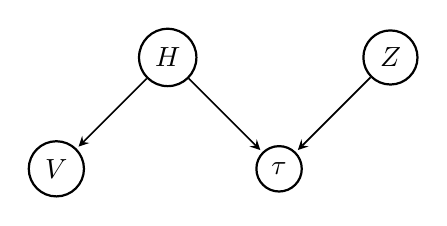
\begin{tikzpicture}[
  > = stealth,
  shorten > = 1pt,
  auto,
  node distance = 2cm,
  semithick
  ]

  \tikzstyle{every state}=[
  draw = black,
  thick,
  fill = white,
  minimum size = 2mm
  ]

  \node[state] (Z) {$Z$};
  \node[state] (t) [below left of=Z] {$\tau$};
  \node[state] (H) [above left of=t] {$H$};
  \node[state] (V) [below left of=H] {$V$};

  \path[->] (Z) edge node {}(t);
  \path[->] (H) edge node {}(t);
  \path[->] (H) edge node {}(V);

\end{tikzpicture}
\vspace{5mm}

Where $H$ is unobserved, $\tau$ is the treatment effect of interest, and $Z$ and $V$ are both observed variables used in a model $f(Z, V)$ that is used to predict $\tau$.
%
Data is simulated according to the following linear structural model:
%
\begin{align*}
y_i &= \tau_i W_i + \epsilon_i \\
\tau_i &= \alpha V_i + \delta H_i \\
Z_i &= \mathcal{N}(Q_{\D}, R_{\D}) \\
V_i &= C_{\D} H_i + \mathcal{N}(J_{\D}, K_{\D}) \\
H_i &= \mathcal{N}(A_{\D}, B_{\D})
\end{align*}
%
Where $\D \in \{1,...,P\}$ indexes the domain in which the data was generated. The following three scenarios are considered:

\begin{enumerate}
\item $A_{\D}, B_{\D}$ are constant across all domains.
\item $A_{\D}, B_{\D}, C_{\D}, J_{\D}, K_{\D}$ and are constant across all domains.
\item None of the above is constant across all domains.
\end{enumerate}

Similarly, the data will be considered in a high-dimensional variant where $V$, $Z$, and $H$ are replaced with groups of variables and a low dimensional variant where they are single variables. The proposed model will be compared with the following baseline techniques:

\begin{enumerate}
\item LASSO on the pooled contexts (\cite{tibshirani1996regression})
\item Model selection via Invariant Prediction (\cite{Peters2015}) followed by OLS on the pooled contexts.
\item Invariance for Causal Transfer Learning (\cite{Rojas-carulla2018}).
\end{enumerate}

\subsection{ Expected Results }

Results will be considered for improvement over baseline models when predicting the oracle treatment effect in target domain $P$ when trained on domains $\{1,...,P-1\}$. The following dimensions will be compared:

\begin{enumerate}
\item Out-of-sample MSE.
\item Percentage of simulations in which the model delivers a positive out-of-sample R-squared.
\item Confidence interval accuracy.
\end{enumerate}

Initial results suggest that a preliminary version of the proposed model show a 12\% improvement in MSE over LASSO when predicting the oracle treatment effect in a left-out target domain in scenario 1.

I expect the proposed model to outperform LASSO on pooled data in scenarios 1 and 3 where the information on the differences between contexts allows the model to penalize more severely unreliable predictors than the LASSO would penalize based on their variance alone. It should perform comparably to LASSO in scenario 2, where all variables should be used in prediction.

The Invariant Prediction (IP) method is inherently conservative, and thus should perform extremely well in scenario 3 where the correct model will not try to use any covariates for prediction. The proposed model will not be as strict, basing its selection on a continuous regularization parameter, but should perform comparably. It should outperform IP in scenario 1 and 2, however, where the conservativeness of IP prevents the model from using available information to make the predictions.


\section{ Chapter 2: Predicting Treatment Effects in a New Context: A Non-Linear Decision Tree Model }

\subsection{ Introduction }

A regression tree is a well-known technique for building a non-linear model between a potentially high-dimensional set of input covariates and a continous target variable. For an introduction and detailed explanation of regression trees and the basic CART (Classification And Regression Tree) algorithm, see \cite{}.

I will assume a basic understanding of the CART algorithm for the remainder of this article. For my purposes, the CART algorithm has several noteworthy properties:

\begin{enumerate}
\item It optimizes over the discrete space of covariates and their interactions with a local, greedy, forward search.
\item It discretizes the continuous input space of covariates.
\end{enumerate}

The optimization implementation implies that at every split of the tree-building process, the CART algorithm is solving the discrete variable selection problem locally based on a defined loss function. Thus, if one can incorporate into the loss function a concept of \textit{domain stability} of the conditional output distribution, the algorithm will pick covariates for which that stability is satisfied locally. This can be contrasted with, for example, a linear model in which the instability of a coefficient across contexts might be driven by only one portion of the input space, whereas the conditional distribution in question might be locally stable in another part. The fact that the algorithm chooses covariates (as opposed to, for example, combining or penalizing them) is attractive in a context where the covariates are thought of as concrete measurements of separable factors that relate somewhat independently to a true underlying causal model\footnote{This feature might also be considered unattractive if one believes that the true causal model operates entirely in a latent space which is jointly dependent on all the input variables.}.

The discretization of the continuous input space of covariates allows for extremely tractable theory regarding treatment effect measurement as well as elegant handling of mixed discrete and continuous covariates.

Finally, regression trees provide a reasonable foundation on which to build a model for domain transfer of treatment effects because of the recent success of Causal Trees (\cite{Athey2016}) and their uptake in both epidimiology and the social sciences. Causal trees allow for non-linear estimation of heterogeneous treatment effects. Heterogeneous treatment effects, being the conditional treatment effect distribution conditional on observed covariates, necessarily form the basis for a transfer model which hopes to transfer to domains in which ovservable covariates differ in distribution.


\subsection{ Literature Review }

The Classification and Regression Trees (CART) algorithm is canonically referenced to the original book:  \cite{breiman1984classification}, however I would direct a reader without familiarity in the topic to more comprehensive books that put decision trees in the context of other statistical algorithms (i.e. \cite{bishop2006pattern}). Bishop explains how decision trees use greedy optimization to pick a series of partitions of the input space, in which an individual, very simple, model makes the prediction (for example, the mean response of that partition might be the prediction in a regression tree). The greedy algorithm is the solution provided to overcome the combinatorial problem of the exponential number of ways that a feature space can be divided by recursive binary splits. To overcome local optima, trees are grown to a large depth and later pruned, allowing for initially poor splits to lead to fruitful nodes.

Causal Trees (\cite{Athey2016}) extend decision trees in two ways: A) they formulate a version of trees to be used with treatment effect data and B) they provide a sample splitting method (``honest estimation'') that provides unbiased estimates and, therefore, accurate confidence intervals through variance prediction of the mean.

More than simply extending decision trees, Causal Trees provided the treatment effect community a disciplined way to deal with the multiple testing problem in heterogeneous effect estimation. The insight comes from understanding that the multiple testing problem for coefficient inference is a direct reflection of the overfitting problem for prediction. Thus, the techniques used to prevent predictive overfitting by CART can, in turn, be used to prevent the multiple testing problem in a posterior heterogeneous effect discovery.

\subsection{ Novelty }

This article extends both the algorithm and the theory of Causal Trees (\cite{Athey2016}) to domain transfer: allowing the algorithm to explicitly incorporate data from multiple domains so as to minimize the predicted error in a new domain.

Results from simulated and real-world data show that the proposed model outperforms Causal Trees, which would otherwise be a state-of-the-art technique for learning the heterogeneity of treatment effects in one context in order to predict the effect of applying the treatment in a new context.

Additionally, this article extends the technique developed in the previous chapter for domain transfer of treatment effects by incorporating the search of high-dimensional linearities directly into the model optimization and allowing the model to use covariates locally for which the predicted treatment is stable only locally.

\subsection{ Theoretical Framework }


The goal is to create an estimator ($\hat{\tau}(x)$) of the true individual treatment effect ($\tau_i$) that minimizes some loss function in new prediction context, given labelled data in a different prediction context. We will consider the squared loss function:
%
$$
\ell(\hat{\tau}, x_i, \tau_i) = (\tau_i - \hat{\tau}(x_i))^2
$$
%
Which will be equivalent to the formulation of causal trees (\cite{Athey2016}). We will similarly create discrete partitions in the feature space such that:
%
$$
\mathcal{X} = \bigcup\limits_{i=1}^{P} \Pi_i
$$
%
And define the following estimator:
%
$$
\hat{\tau}(x, \Pi, S(\D)) =  \bar{y}^1_i - \bar{y}^0_i \ \ ; x \in \Pi_i\ ; \ i : x \in \Pi_i
$$
%
Where $S(\cdot)$ consists of a sampling function to sample matched data $(y, x)$ from a domain $\D$. $\Pi$ consists of some particular partitioning of the feature space. As the sample mean is an unbiased estimate of the expectation, this is an unbiased estimate of $\tau(x,\Pi, \D) \coloneqq \mathbb{E}[\tau | X \in \Pi_i ]$. We would like to minimize our expected loss:
%
$$
\Ex \ell(\Pi) = \Ex_{X, S} [ (\tau_i - \TTs^2  ]
$$
%
Where our expectation is taken over all potential samples data in our source domain, $S(\D_S)$ and all the potential target data points, $X$. We can expand this loss function:
%
$$
\Ex \ell(\Pi) = \underbrace{\Ex_{X} [ \tau_i^2]}_{\text{doesn't depend on $\Pi$}} - 2 \Ex_{X, S}[ \tau_i\TTs] + \Ex_{X}[  \Ex_{S} [\TTs^2 ]]
$$
%
We can expand the middle term with the law of iterated expectations and note that, conditional on the value being within a leaf, $\tau_i$ and $\TTs$ become independent:
%
\begin{align*}
&-2 \Ex_{X,S}[ \underbrace{\Ex_{X}[ \tau_i | x_i \in \Pi_i]}_{= \tau(x_i, \Pi, \D_T)} \ \underbrace{\Ex_{S} [ \TTs | x_i \in \Pi_i]}_{= \tau(x_i, \Pi, \D_S)}] ] + \Ex_{X}[  \Ex_{S} [\TTs^2 ]]\\
&-2 \Ex_{X}[ \tau(x_i, \Pi, \mathcal{D}_T)  \tau(x_i, \Pi, \mathcal{D}_S) ] + \Ex_{X}[  \Ex_{S} [\TTs^2 ]]
\end{align*}

Where we can see that this objective function has some interpretable properties: we wish to maximize the cross product of the actual average treatment effect in the source and target domain, given a particular partition, without increasing the square product of our predicted treatment effect for that partition. This chapter will solve for a sample estimate of the above objective function and test it empirically.

\subsection{ Data Simulation }

Data reflects a true causal model given by the following directed acyclic graph in:

\vspace{5mm}
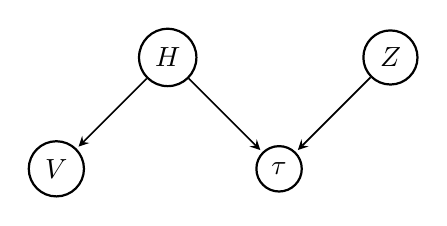
\begin{tikzpicture}[
  > = stealth,
  shorten > = 1pt,
  auto,
  node distance = 2cm,
  semithick
  ]

  \tikzstyle{every state}=[
  draw = black,
  thick,
  fill = white,
  minimum size = 2mm
  ]

  \node[state] (Z) {$Z$};
  \node[state] (t) [below left of=Z] {$\tau$};
  \node[state] (H) [above left of=t] {$H$};
  \node[state] (V) [below left of=H] {$V$};

  \path[->] (Z) edge node {}(t);
  \path[->] (H) edge node {}(t);
  \path[->] (H) edge node {}(V);

\end{tikzpicture}
\vspace{5mm}

Where $H$ is unobserved, $\tau$ is the treatment effect of interest, and $Z$ and $V$ are both observed variables used in a model $f(Z, V)$ that is used to predict $\tau$.
%
Data is simulated according to the following non-linear structural model:
%
\begin{align*}
y_i &= \tau_i W_i + \epsilon_i \\
\tau_i &= \alpha V_i \cdot  1 \{ V_i > \gamma \} + \delta H_i \cdot  1 \{ H_i > \phi \}\\
Z_i &= \mathcal{N}(Q_{\D}, R_{\D}) \\
V_i &= C_{\D} H_i + \mathcal{N}(J_{\D}, K_{\D}) \\
H_i &= \mathcal{N}(A_{\D}, B_{\D})
\end{align*}
%
Where $\D \in \{1,...,P\}$ indexes the domain in which the data was generated. The following three scenarios are considered:

\begin{enumerate}
\item $A_{\D}, B_{\D}$ are constant across all domains.
\item $A_{\D}, B_{\D}, C_{\D}, J_{\D}, K_{\D}$ and are constant across all domains.
\item None of the above is constant across all domains.
\end{enumerate}

Similarly, the data will be considered in a high-dimensional variant where $V$, $Z$, and $H$ are replaced with groups of variables and a low dimensional variant where they are single variables. The proposed model will be compared with the following baseline techniques:

\begin{enumerate}
\item Causal Trees (\cite{Athey2016})
\item Proposed Linear Model from Chapter 1
\end{enumerate}



\subsection{ Expected Results }

Results will be considered for improvement over baseline models when predicting the oracle treatment effect in target domain $P$ when trained on domains $\{1,...,P-1\}$. The following dimensions will be compared:

\begin{enumerate}
\item Out-of-sample MSE.
\item Percentage of simulations in which the model delivers a positive out-of-sample R-squared.
\item Confidence interval accuracy.
\end{enumerate}

The nonlinearties of the treatment effects in the data generating process should cause the linear model to perform suboptimally compared to the tree-based models, which can directly learn the break points that cause the non-linearities in the simulated data. This should especially reflect in the first two performance measures.

I expect the proposed model to outperform Causal Trees in scenarios 1 and 3 where the information on the differences between contexts allows the model to penalize more severely unreliable predictors than Causal Trees would penalize based on their variance alone. Initial results on scenario 1 bear this out, with a close to 20\% improvement in MSE.

In scenario 2, I expect both models to perform poorly, but the proposed model should be more conservative than the causal trees and the confidence intervals of its predictions should reflect the cross-domain variance in conditional distributions, thus providing greater confidence interval accuracy than the Causal Trees would provide from considering the pooled variance alone.

\section{ Chapter 3: Predicting the Effects of Unconditional Cash Transfer Programs Across Countries }

\subsection{ Introduction }

Transferring cash has always been the most straight forward way to implement redistribution. While conditional cash transfer programs require the participants to either participate in some activity (looking for work) or spend the money is a certain fashion (on food), unconditional cash transfer (UCT) programs put no restrictions on the use of the money or behavior of the recipient. Unconditional cash transfers have gained increasing interest in recent times in two different spheres of influence: A) as poverty reduction scheme in low- and middle-income countries, where 130 countries now have some UCT program (\cite[see][for a comprehensive overview]{Bastagli2016}) and B) in the form of a Universal Basic Income in high-income countries (\cite[see]{Hoynes2019}).

Potential outcomes and treatment effect frameworks (see \cite{imbens2015causal} for an overview) have been extremely successful in areas such as medicine. In medicine, the stable unit treatment value assumption is often trivially satisfied, the operating context (the human body) is constant across time, space, and political organization, and the treatment (i.e. the drug) is reproduced identically between trial and deployment into the real world.

The same cannot, unfortunately, be said for the social sciences and in particular economics. Despite the great prevalence of treatment effect studies and counterfactual inference, it is far from straight forward to generalize from a successful policy in one country to its implementation in another. Regarding economic policies, both the context (with all its supporting variables) and the treatment (with all its nasty details) cannot be kept identical (\cite{Cartwright2013}).

Despite these challenges, prediction of treatment effects is a required part of the normative aspect of the economics profession, and will be for as long as economists believe they have anything to contribute to public policy. One cannot recommend a policy without some implicit or explicit prediction of its effect in the predictive context. If one is informed in any way in their recommendation by past studies of similar policies in other contexts, then one is making, either formally or through the wanderings of a creative imagination, a prediction of a treatment effect in a new context given past results in a different one.

Thus, predicting treatment effects in a new context is a task unavoidable for the policy maker or anyone involved in advising. Despite its difficulties, however, we also have reason to believe it is possible: humans must have some traits in common across countries and time periods, market economies share some similarities, and policies that look similar in relevant aspects will likely have similar effects on the actions of those citizens effected by their implementation.

In particular, despite its differences, poverty shares many similarities across countries: it consists of a lack of ability to purchase desired goods, it's undesirable, and it's a condition experienced by some but not all people in a society. Similarly, the choice to work, despite all the many other differences, still involves a tradeoff between desire for greater purchasing power and desire for leisure time. Finally, domestic labor and labor sharing arrangements, while it may vary in scope from country to country, is largely free of monetary exchange.

As such, the core concerns and questions surrounding policies of unconditional cash transfers to those in poverty share similar concerns: Does it reduce the incentive to work outside of the home? Does it increase the incentive to work inside the home? What would the effects be on the labor supply and how would that effect our economy? What are the effects be on the psychological well being of the individuals who recieve the transfer?

On the other hand, the choice to work outside the home is only a choice as so far as there are employment opportunities available, the choice to work inside the home may be dictated more by societal gender norms than anything to do with spending power, and work itself may bring benefits outside of income that differ greatly from context to context.

The transferability of knowledge regarding UCT is, therefore, a prior ambiguous. As such, UCT provides an interesting test bed for treatment effect prediction because there is both data from widely different contexts (from Canada in the 1970s to Mexico in the 2000s to Finland in the 2010s) and the transferability of findings from one context to another is highly ambiguous and very potentially impossible.

\subsection{ Literature Review }

Studies (experiments) on UCT programs can be classified broadly into two groups:

\begin{enumerate}
\item Basic income experiments in high-income countries. For example, experiments in North America between 1968-1978 (\cite{Forget2011}) and those in Europe since 2016, such as a 2-year pilot program in Finland from 2017-2019 (\cite{Kangas2019}) and a similar pilot program in Utrecht in the Netherlands (currently in progress).

\item Poverty-assistance UCT programs in low- and middle-income countries since 2000. A good overview of these studies (both conditional and unconditional) is provided by Banerjee et al \parencite*{Banerjee2017}. This includes, among others, several programs by the NGO GiveDirectly (\cite{Blattman2016}), the PAL program for rural villages in Mexico (\cite{Cunha2019}), which compared cash to in-kind transfers of food), and a UCT program in Madhra Pradesh, India (\cite{bharat2014little}).

\end{enumerate}

It is telling that, in a recent symposium they organized on UBI, the Annual Review of Economics published two entirely separate reports: one on the US and ``advanced'' countries, another on the ``developing world'' (\cite{Hoynes2019, Banerjee2019}). Which is to say, when reviewing the evidence and discussing potential policies related to UBI, they saw it beneficial to consider the two contexts and separate problems entirely, implying that what one learns in one most likely has very little to do with the other.

Despite that, many proponents of UBI will cite UCT studies from low- and middle-income countries as evidence that ``people act in their own interest when given free cash'' (\cite{van2017basic}). From a definitional perspective, UBI is unequivocally a form a unconditional cash transfer. It has other defining characteristics, some of which are not entirely agreed upon (\cite{Hoynes2019}), but Banerjee et al \parencite*{Banerjee2019} lays out several dimensions on which the majority of UBI proposals differ from the majority of UCT experiments in low- and middle-income countries:

\begin{enumerate}
\item Universality. Very few studies (of any kind, including those that explicitly study basic income) can, by their very nature, test a truly universal basic income. The universality of the program can lead to effects on labor markets that small trials cannot hope to explore. One recent study (\cite{Egger2019}) seeks to explore the general equilibrium effects of cash transfers, which is an important step in the direction of understanding the effects of universality, however they still only tested the effect of giving cash to a small set of families (their novelty is in the measurement of the effects that goes beyond those families).

Additionally, universality is often different from UCT programs in low- and middle-income countries in that it implies the participation of all people, not just the poorest ones. This relates to a lot of interesting but complex psychological ideas (such as stigma) that relate to receiving aid from the government. These issues, similarly, have not been able to be tested in any experiment until now.
\item Duration. Few studies are able to continue giving cash for a long period of time. That being said, in theory the UCT programs being trialed in low- and middle-income countries would be continued indefinitely if successful.
\item Amount. Most basic income proposals suggest that the amount of cash should be relatively high, enough to live on. This is not always the case with UCT programs in low- and middle-income countries where the cash is just meant to ``help.''
\end{enumerate}

For my purposes, universality and duration are not features we can easily test without further structure. For the purposes of this study, therefore, I consider UBI experiments to be UCT experiments that may or may not offer a different amount of purchasing power and that, most interestingly, take place in a different context.

Despite the fact that many of the interesting societal effects of a UBI program cannot be tested, there is a narrower effect on the individual level, that one could potentially imagine fulfills the stable unit treatment value assumption: the effect that receiving extra cash has on ones desire to participate in a (fixed) labor market.

This is a major policy outcome concern for unconditional cash transfers (\cite{Hoynes2019}). Specifically, will labor supply decrease if cash transfers provide a source of income other than labor? Most studies of UCT programs record labor market participation for this reason.

The only meta-analysis that I am aware of which uses the full microdata from various UCT studies to analyze the effect of unconditional cash on labor market participation was conducted recently by Banerjee et al \parencite*{Banerjee2017}. They extend a pooled OLS analysis by using a Bayesian hierarchical framework, treating the treatment effect parameter of each study $\tau_S$ as a normally distributed random variable whose mean and variance are estimated via Hamiltonian Markov Chain Monte Carlo. They find that the effect of cash transfer on the probability of working is centered at zero for men (slightly negative, -0.01, for woman), with 95\% of probability mass from -0.02 to -0.03 for men (-0.04 to 0.02 for women).

\subsection{ Novelty }

This research seeks to contribute to the literature in two separate ways:

\begin{enumerate}
\item Provide a systematic meta-analysis, from microdata, of a series of unconditional cash transfer RCT's that have not been previously compared in such a way. As such, it contributes to the understanding of this policy and its similarities and differences across contexts. In particular, it will contribute in two particular ways due to the statistical nature of the technique used: A) understanding the heterogeneous effects these policies have on individuals and B) understanding which of those effects are most stable across space and time.

\item Provide a test bed of a new technique, that developed in Chapter 1 and 2 of this thesis, on an interesting real world problem. As this problem is uniquely large in scope (spanning vastly different countries and time periods), it provides an opportunity to test the ``transfer limits,'' showing that the new proposed technique manages to ``fail gracefully'' and quantify uncertainty accurately across changes in context so large that learning is potentially impossible.
\end{enumerate}

By comparing the results of the proposed technique (chapter 2) to a baseline consisting of the hierarchical model presented in Banerjee et al \parencite*{Banerjee2017}, I seek to contribute a clear comparison of techniques. I expect that my proposed technique performs better than their hierarchical model, as their treatment effects are allowed to vary around a mean, but they do not attempt to explain the variation, neither via study-level variables or individual-level variables, and similarly do not learn any heterogeneous treatment effects.

\subsection{ Theoretical Framework }

The potential outcomes framework has a history going back to Jerzy Neyman, but Donald Rubin revived the ideas and formalized them in a modern form in the 1970s and 80s and Paul Holland \parencite*{Holland1986} wrote a landmark paper that is often referenced as the formalization of the entire framework which is most used. Before formulating the model, Holland starts the paper by framing his goal:

\begin{displayquote}
``Others are concerned with deducing the causes of a given effect. Still others are interested in understanding the details of causal mechanisms. The emphasis here will be on measuring the effects of causes because this seems to be a place where statistics, which is concerned with measurement, has contributions to make.''
\end{displayquote}

The success of Fisher's framework of randomization and the Rubin-Neyman causal model comes down to this razor focus in purpose: they make no claims to discover all the causes of a given effect, to discover the mechanism of the cause, or even to separate between a cause or a necessary part of a cause. They allow us to reason about counterfactuals: what would have happened, on average and in the past, had we treated our entire population rather than a randomized part of a randomized sample drawn from that population. It operationalizes John Stuart Mill's method of differences, creating a pathway to internal validity that is achievable in the real world.

The potential outcomes framework considers the outcomes for a particular individual, $y_i$ as one of two possible ``potential'' outcomes, unique to that individual:
$$
y_i = (w_i)y^1_i + (1 - w_i)y^0_i
$$
Where $y^1_i$ and $y^0_i$ represent the ``potential'' outcomes that individual $i$ would experience under treatment ($w_i = 1$) and control ($w_i = 0$), respectively.

One important assumption embodied by this equation is known as the Stable Unit Treatment Value assumption: that each individual's outcome is only effected by their own treatment status, and not the treatment status of anyone else. This assumption is especially important in the context of cash transfers. In particular, if one believes that an individual's experience of money and welfare programs is in any way relative or socially contextualized, this assumption is violated.

Despite that potential violation of assumptions, I will stick to the potential outcomes framework for this study. This is due to A) the acceptance of this assumption in prior art regarding this topic and B) the lack of well-known alternatives.

Given this framework for the outcome of an individual, it's natural to ask about the ``treatment effect'' on the individual, defined as:
$$
\tau_i = y^1_i - y^0_i
$$
Unfortunately, as by definition one can never observe the counterfactual outcomes $y^1$ and $y^0$ for the same person, the treatment effect $\tau_i$ is unobservable. This is referred to as ``the fundamental problem of causal inference'' by Paul Holland \parencite*{Holland1986}.

Consider a policy maker that would like to decide on applying a particular treatment to her population by comparing the distributions of outcomes if she had applied the treatment, $P(Y^1)$, to the distribution of outcomes had she not applied the treatment, $P(Y^0)$. Unfortunately, by definition of how we defined the potential outcomes, one can only ever observe $P(Y^1 | W = 1)$ and $P(Y^0 | W = 0)$. This problem is overcome via the ``unconfoundedness assumption''.

The unconfoundedness assumption requires that one create a dataset in which $P(Y^1) = P(Y^1 | W = 1)$ and $P(Y^0) = P(Y^1 | W = 0)$. Trivially, in the data considered in this study, that is achieved via randomization of $W$ such that it is assumed independent of the potential outcomes.


\subsection{ Econometric Estimation }

The purpose of this article is to test the accuracy of predicting the treatment effect of a new cash transfer program in a country or context in which one has no previous data or experiments.

Given a set of ``source contexts'' (studies), I will test the accuracy of several potential predictive models to predict the treatment effect on a held-out ``target context'' (a separate study in a different country and/or time).

I consider the treatment to be the cash transfer itself. I consider three outcomes: part-time employment, full-time employment, and health.

Finally, I consider the following predictive models:

\begin{enumerate}
\item The ATE estimated by OLS on the pooled data of source contexts.
\item The MAP estimate from a Bayesian hierarchical model trained on the source contexts, where the treatment effect is allowed to vary across contexts according to a normal distribution of learned mean and variance (\cite{}).
\item Causal Trees trained on the pooled data of source contexts.
\item The proposed model from chapter 2.
\end{enumerate}

In simulating data, one can test techniques against the so-called ``oracle'' treatment effect: the true treatment effect that was simulated for that individual. In the real world, however, treatment effects cannot be measured, as per the ``fundamental problem of causal inference'' (\cite{}).

There are several potential strategies for overcoming this problem and measuring the loss of the predicted treatment effect for each individual, as predicted by model $\tau^*(x_i)$:

\begin{enumerate}
\item Use the partitioning scheme ($\Pi$) of the tree-based model directly, such that the loss for a particular individual in the target context is given by:
%
\begin{align*}
&\hat{\tau}(x, \Pi, S(\D)) =  \bar{y}^1_i - \bar{y}^0_i \ \ ; x \in \Pi_i\ ; \ i : x \in \Pi_i \\
&\ell(y_i, x_i) = \big(\hat{\tau}(x_i, \Pi, S(\D_{T})) - \tau^*(x_i) \big)^2 \\
&\mathbb{E}\ell(y_i, x_i) \approx \frac{1}{N} \sum_i \big(\hat{\tau}(x_i, \Pi, S(\D_{T})) - \tau^*(x_i) \big)^2
\end{align*}
%
The downside of this strategy is that the ``target value'' is not independent of the partitioning scheme learned by the model.

\item Use a matching function ($f(\cdot)$) to create an estimate of the individual treatment effect on the treated and compare that with the effect predicted by the model:
%
\begin{align*}
\ell(y_i, x_i) = \big( (y^1_i - y^0_{f(x_i)} ) - \tau^*(x_i) \big)^2
\end{align*}

Which has the advantage of comparing to a target value which is fully independent of the model used in prediction. The disadvantage is that the predicted treatment effect, $(y^1_i - y^0_{f(x_i)} )$ is limited in accuracy to the matching function's ability to choose the optimum feature space ($x_i$) and distance. Indeed, this is the exact optimization problem that CART models solve.

\item Use an estimate of the treatment effect provided by a partitioning ($\Pi_T$)learned by the Causal Trees algorithm trained solely on the training data:
\begin{align*}
&\hat{\tau}(x, \Pi, S(\D)) =  \bar{y}^1_i - \bar{y}^0_i \ \ ; x \in \Pi_i\ ; \ i : x \in \Pi_i \\
&\ell(y_i, x_i) = \big(\hat{\tau}(x_i, \Pi_T, S(\D_{T})) - \tau^*(x_i) \big)^2 \\
&\mathbb{E}\ell(y_i, x_i) \approx \frac{1}{N} \sum_i \big(\hat{\tau}(x_i, \Pi_T, S(\D_{T})) - \tau^*(x_i) \big)^2
\end{align*}
%
This has the advantage that the partitioning and therefore the ``target value'' is independent of the learned model, as well as providing a prediction of the ``target value'' that handles explicitly the feature space problem provided by $X$. Given these advantages, I will use this strategy to evaluate the accuracy of the predictive models.

\end{enumerate}


\subsection{ Expected Results }

Given that the proposed prediction technique explicitly minimizes an expected predicted loss in a new context, it is reasonable to believe that the mathematical theory will bear out to some degree in real world data and that the proposed technique will outperform the other three baseline techniques in predicted error applied to the effect of cash transfers.

While there is no current study of these particular cash transfer projects on which to base an expectation of the transferability of results across contexts, basic economic theory, as mentioned previously, would suggest that the fundamental tradeoff between consumption, investment, and leisure is shared across contexts and that could very well provide the basis to predict reasonably across context. With that in mind, I expect the model to return a positive R-squared in predicting in some target contexts, providing a better prediction for the individuals of the target context than the mean treatment effect in that context, and showing that there is a model of heterogeneous treatment effects that explains a large part of the effect of this treatment on employment. Conversely, I expect the model will fail to predict effectively in one or more target contexts, showing the limits of model transfer with policies as complex as cash transfers.



% Say something about being able to predict the results better than a mean and the implications for policy-making



% \section{ Chapter 3: Mixed-Causality Representation Learning for Domain Transfer  }

% The true causal model of a particular outcome variable is believed to exist entirely on a latent space.

% You have a set of variables that you believe to be potentially correlated with the latent causal variables.

% Some of those variables might be causes, some might be effects, potentially even, some might be both (simultaneity).

% In a traditional prediction task, a network is learned to predict the outcome, the transformations necessary to go from covariate to outcome treated as an uninteresting black box.

% However, given a causal model, one believes that certain variables cause the latent variables and others are caused by them. This is important for determining which variables to use in the prediction if one changes domain.

% The idea is to learn the causal and the caused variables, like an autoencoder. In theory, that would produce a causal model which transfers well across domains by only using the causal variables, as well as a test for domain transferability by the prediction failure of the model on the caused variables.

%
%


% \section{ Chapter 3: Recovery of latent sub-contexts in treatment effect data for use in out-of-context prediction }

\printbibliography

\appendix

\section { Working Schedule }


\textbf{Q1 2020}

\begin{itemize}
\item (Chapter 1) Create initial, flexible pytorch framework for implementing optimization.
\item (Chapter 1) Create first proposal of simulation data that can be used to test model.
\item (Chapter 1) Create first proposal of objective function.
\item (Chapter 2) Create flexible and eficient Python framework for decision tree models. Reproduce causal trees and all results from their paper.
\item (Chapter 2) Implement initial proposal of “Causal Transfer Tree” in above framework.
\item (Chapter 2) Create first proposal of simulation data that can be used to test model.
\item (Chapter 2) Create first proposal of objective function and vet feasibility of a workable solution.
\end{itemize}


\textbf{Q2 2020}

\begin{itemize}
\item (Chapter 1 \& 2) Solve initial proposed objective function and implement in model.
\item (Chapter 1 \& 2) Document results over simulation data of proposed objective function. Compare to alternatives.
\item (Chapter 1 \& 2) Write up results of model and simulations into draft of a working paper.
\item (Chapter 1 \& 2) Present current model 2-3 times to groups of economists and statisticians.
\end{itemize}


\textbf{Q3 2020}

\begin{itemize}
\item (Chapter 1 \& 2) Test models and understand performance on simple real world data (microcredit) and write up new versions of model to perform better.
\item (Chapter 2) Create new simulation dataset that exemplies a new aspect of the problem seen in the real world data.
\item Identify potential research stay and research group that might help the development of the project.
\end{itemize}


\textbf{Q4 2020}

\begin{itemize}
\item Identify (2) extensions of the model(s) that could be researched by BGSE master’s students for theses in 2021.
\item (Chapter 1 \& 2) Submit chapters as an article to a reasonable econometric journal.
\item Present current work at 1-2 conferences.
\end{itemize}

\textbf{Q1 2021}

\begin{itemize}
\item (Chapter 3) Review newly available studies and data from 2020 for inclusion.
\item (Chapter 3) Gather data and create combined dataset from the chosen studies.
\item (Chapter 1 \& 2) Potential research stay with research group that will be helpful to develop third generation of the technique.
\end{itemize}

\textbf{Q2 2021}

\begin{itemize}
\item (Chapter 3) Clean and check all the data from the cash transfer studies.
\item (Chapter 3) Apply tree model to cash transfer studies and document results.
\item (Chapter 1 \& 2) Present technique(s) at 3-4 small-to-midsized conferences.
\item (Chapter 1 \& 2) Prepare, document, and advertise Python package(s). Create Stata extension(s).
\end{itemize}

\textbf{Q3 2021}

\begin{itemize}
\item (Chapter 3) Submit results to 1-2 small conferences
\item (Chapter 1 \& 2) Present technique(s) at 1-2 major conferences.
\item (Chapter 1 \& 2) Re-submit article(s) to 2nd choice journal(s).
\end{itemize}

\textbf{Q4 2021}

\begin{itemize}
\item (Chapter 3) Finish article on empirical results and submit to first-choice applied economics journal.
\item Submit thesis.
\end{itemize}


\section{International Research Stay}

As outlined in the schedule, I aim to participate in an international research stay during or around Q1/Q2 of 2021. These are the following universities and research groups I am currently considering, in order of preference:

\begin{enumerate}
\item University of Copenhagen. Jonas Peters. Copenhagen Causality Lab.
\item ETH Zurich. Nicolai Meinshausen.
\item Max Planck Institute for Intelligent Systems. Bernhard Schölkopf. Department of Empirical Inference.
\end{enumerate}

\section{Doctorat Activities}

I will engage in the following research activites consistently throughout the doctorat process:

\begin{enumerate}
\item Attend PhD seminars in the department of Applied Economics at UAB.
\item Attend Statistics seminars in the department of Economics at UPF.
\item Annual evaluation of the Applied Economics department at UAB.
\end{enumerate}

In addition to those activities, I hope to attend 1-2 relevant summer schools at UAB and potentially abroad. Unfortunately, this is most likely first in 2021 due to Covid-19.

As outlined in the schedule, I will submit and hope to present at a range of conferences and seminars. At this time, I can only name the following for sure:

\begin{enumerate}
\item  International Conference on Economic Modeling and Data Science, EcoMod (Accepted\footnote{Initial draft of Chapter 2 was accepted to the 2020 conference, but the conference was postponed until 2021. Acceptance status is maintained.}).
\item UAB PhD Applied Economics Doctoral Workshop.
\item Statistics Seminar at UPF.
\end{enumerate}
%
I will, however, target the following A-level conferences in 2021:

\begin{enumerate}
\item World Congress of the Econometric Society
\item International Symposium on Econometric Theory and Applications
\item IAAE Annual Conference
\end{enumerate}

\section{Funding}

I will be self-funding my research.




\end{document}
